\chapter{远程火箭飞行的力学环境}
\thispagestyle{empty}
\section{附加力、附加力矩及火箭发动机特性}

\subsection{附加力和附加力矩}
\vspace*{-1em}

\theorem[雷诺迁移定理]
{
	连续运动的流体场中同一部分的流体质点上,标量或矢量点函数的体积分的全导数和该点函数局部导数的体积分之间有如下的关系:
	\begin{equation}
		\dfrac{\d}{\d t}\int\limits_{V} A \, \d V = \int\limits_{V} \dfrac{\partial A}{\partial t} \, \d V+ \int\limits_{S} A(\bm{V} \cdot \bm{n})\, \d S
		\label{雷诺迁移定理}
	\end{equation}
	其中,\vspace*{-0.5em}
	{
		\begin{enumerate}[\hspace*{2em}]
			\item $A$ \quad 标量场或矢量场\vspace*{-0.5em}
			\item $V$ \quad 所研究部分流体的体积\vspace*{-0.5em}
			\item $S$ \quad 所研究部分流体的表面积\vspace*{-0.5em}
			\item $\bm{V}$ \quad 表面$S$上流体质点的运动速度矢量\vspace*{-0.5em}
			\item $\bm{n}$ \quad 表面$S$外法向上的单位矢量
		\end{enumerate}
	}
}

\noindent 设火箭为一轴对称体,定义新物理量如下\vspace*{-0.5em}
\begin{enumerate}[\hspace*{2em}]
	\item $S_e$ \quad 发动机喷管出口截面积\vspace*{-0.5em}
	\item $o_1$ \quad 火箭的质心\vspace*{-0.5em}
	\item $\bm{V}_{rc}$ \quad 燃料燃烧过程中$t$时刻质心$o_1$相对于箭体的运动速度\vspace*{-0.5em}
	\item $\bm{V}_{rb}$ \quad 燃料燃烧过程中$t$时刻某一质点相对于箭体的运动速度
\end{enumerate}
则质点相对于质心的速度为
\begin{equation}
	\dfrac{\delta \vrho}{\delta t} = \vV_{rb} - \vV_{rc}
	\label{dp}
\end{equation}
令$\bm{A} = \rho_m \bm{H}$,则代入雷诺迁移定理\eqref{雷诺迁移定理}可得
\begin{equation*}
	\dfrac{\partial }{\partial t}\int\limits_{V} \rho_m \vH \, \d V =  \int\limits_{V} \dfrac{\partial \rho_m \vH}{\partial t} \, \d V + \int\limits_{S} \rho_m \vH (\bm{V}_{rb} \cdot \bm{n})\, \d S
\end{equation*}
由于$\d V = \dfrac{\d m}{\rho_m}$,则可以得到
\begin{equation}
	 \int\limits_{m} \dfrac{\partial \vH}{\partial t} \, \d m  =  \dfrac{\partial }{\partial t}\int\limits_{m} \vH \, \d m + \int\limits_{S_e}  \vH (\rho_m \bm{V}_{rb} \cdot \bm{n})\, \d S_e
\end{equation}
其中,$\rho_m$为流体质量密度,$\bm{n}$为喷管截面$S_e$外法向矢量,$\bm{H}$为任意的矢量点函数。

利用这个式子,可以得到作用于火箭上的附加力和附加力矩。
\vspace*{1em}

\noindent \textbf{1. 附加相对力}

由附加相对力的定义,
\begin{equation*}
	\bm{F}'_{rel} = - \int_m \dfrac{\delta^2 \vrho}{\delta t^2}\, \d m 
\end{equation*}
在雷诺传输定理中令$\bm{H} = \dfrac{\delta \bm{\rho}}{\delta t}$,可以得到
\begin{equation}
	\bm{F}'_{rel} = - \dfrac{\delta}{\delta t}\int_m \dfrac{\delta \bm{\rho}}{\delta t} \, \d m - \int_{S_e} \dfrac{\delta \bm{\rho}}{\delta t} (\rho_m V_{rb}\cdot \bm{n}) \, \d S_{e}
	\label{附加相对力1}
\end{equation}

由$\dfrac{\delta \bm{\rho}}{\delta t} = \bm{V}_{rb} - \bm{V}_{rc}$对公式\eqref{附加相对力1}右端第二项处理得到
\begin{align*}
	 \int_{S_e} \dfrac{\delta \bm{\rho}}{\delta t} (\rho_m V_{rb}\cdot \bm{n} \, \d m)
	  = \int_{S_e} (\bm{V}_{rb} - \bm{V}_{rc}) (\rho_m V_{rb}\cdot \bm{n}) \, \d S_{e}
\end{align*}
而质心速度$\bm{V}_{rc}$与面积无关,且假设面$S_e$上的质点的速度相同,定义$\bm{V}_{rb} = \bm{\mu}_e$,那么
\begin{align*}
	\int_{S_e} \dfrac{\delta \bm{\rho}}{\delta t} (\rho_m V_{rb}\cdot \bm{n} \, \d m)
	= \int_{S_e} (\rho_m V_{rb}\cdot \bm{n}) \, \d S_{e} (\bm{\mu}_e - \bm{V}_{rc})
\end{align*}
而
\begin{equation*}
	\int_{S_e} (\rho_m V_{rb}\cdot \bm{n}) \, \d S_{e} = \dot{m}
\end{equation*}
其中,$\dot{m}$为\dy[质量秒耗量]{ZLMHL},则最终简化为
\begin{equation}
	\int_{S_e} \dfrac{\delta \bm{\rho}}{\delta t} (\rho_m V_{rb}\cdot \bm{n} )\, \d m
	= \dot{m}\bm{\mu}_e - \dot{m} \bm{V}_{rb}
\end{equation}
若截面上每个点的速度不相等,可以重新定义$\bm{\mu}_e$为
\begin{equation}
	\bm{\mu}_e = \dfrac{1}{\dot{m}}\int_{S_e}\bm{V}_{rb} (\rho_m V_{rb}\cdot \bm{n}) \, \d S_{e}
\end{equation}

对于公式\eqref{附加相对力1}右端第一项,在雷诺运输方程中令$\bm{H} = \bm{\rho}$,可以得到
\begin{equation*}
	\int_m \dfrac{\delta \bm{\rho}}{\delta t} \, \d m= \dfrac{\delta}{\delta t}\int_m \bm{\rho} \, \d m + \int_{S_e}  \bm{\rho}  (\rho_m V_{rb}\cdot \bm{n}) \, \d S_{e} =  \int_{S_e}  \bm{\rho}  (\rho_m V_{rb}\cdot \bm{n}) \, \d S_{e} 
\end{equation*}
喷口截面上任意一点矢量$\bm{\rho}$为火箭质心$o_1$到截面中心矢量$\bm{\rho}_e$与截面中心到该点到矢量$\bm{\nu}$之和,如图所示。即
\begin{equation}
	\bm{\rho} = \bm{\rho}_e + \bm{\nu}
\end{equation}
如果喷口处质点速度相同,且喷口对称,则
\begin{equation*}
	\int_{S_e}  \bm{\nu}  (\rho_m V_{rb}\cdot \bm{n}) \, \d S_{e} 
\end{equation*}
则公式\eqref{附加相对力1}右端第一项最终简化为
\begin{equation}
		\int_m \dfrac{\delta \bm{\rho}}{\delta t} \, \d m= \int_{S_e}  \bm{\rho}_e  (\rho_m V_{rb}\cdot \bm{n}) \, \d S_{e}  = \dot{m}\bm{\rho}_e
		\label{质量秒耗量}
\end{equation}
若截面上每个点的速度不相等,可以重新定义$\bm{\rho}_e$为(平均中心)
\begin{equation}
	\bm{\rho}_e = \dfrac{1}{\dot{m}}\int_{S_e}\bm{\rho} (\rho_m V_{rb}\cdot \bm{n}) \, \d S_{e}
\end{equation}
所以可以得到

\theorem[附加相对力]
{
	\vspace*{-1em}
	\begin{equation}
		\bm{F}'_{rel} = - \ddot{m}\bm{\rho}_e - \dot{m}\dot{\bm{\rho}_e} - \dot{m}\bm{\mu}_e + \dot{m}\bm{V}_{rc}
	\end{equation}
	\hspace*{2em} 考虑到火箭质点流动的非定常性很小,且质心变化速度$\bm{V}_{rc}$及喷口中心矢径$\bm{\rho}_e$的变化很小,因此有附加相对力为:
	\begin{equation}
		\bm{F}'_{rel} = - \dot{m}\bm{\mu}_e
	\end{equation}
	其中,\vspace*{-0.5em}
	{
		\begin{enumerate}[\hspace*{2em}]
			\item $\dot{m}$ \quad 质量秒耗量\vspace*{-1em}
			\item $\bm{\mu}_e$ \quad 喷口截面平均速度
		\end{enumerate}
	}
}
\vspace*{0.5em}

\noindent \textbf{2. 附加哥式力}

由\peref[运动方程]可以得到附加哥氏力的表达式为
\begin{equation*}
	\bm{F}'_k = - 2 \bm{\omega}_T \times \int_m \dfrac{\delta \bm{\rho}}{\delta t} \, \d m
\end{equation*}
将$\displaystyle \int_m \dfrac{\delta \bm{\rho}}{\delta t}\, \d m = \dot{m}\bm{\rho}_e$代入可以得到

\theorem[附加哥氏力]
{
	\vspace*{-1.5em}
	\begin{equation}
		\bm{F}'_k = - 2 \dot{m}\bm{\omega}_T \times \bm{\rho}_e
	\end{equation}
}

\vspace*{0.5em}

\noindent \textbf{3. 附加哥式力矩}

由\peref[绕质心的运动方程]可以得到附加哥氏力矩的表达式为
\begin{equation}
	\bm{M}'_k = - 2 \int_m \bm{\rho}\times \left(\bm{\omega}_T \times \dfrac{\delta \bm{\rho}}{\delta t}\right)\, \d m
\end{equation}
由复合求导法则及向量叉乘的运算律,可以得到
\begin{equation*}
	\begin{cases}
		\, \dfrac{\delta }{\delta t} [\bm{\rho} \times (\bm{\omega}_T \times \bm{\rho})] = \dfrac{\delta \bm{\rho}}{\delta t} \times (\bm{\omega}_T \times \bm{\rho}) + \bm{\rho} \times \left(\dfrac{\d \bm{\omega}_T}{\d t} \times \bm{\rho}\right) + \bm{\rho}\times \left(\bm{\omega}_T \times \dfrac{\delta \bm{\rho}}{\delta t}\right) \\[0.8em]
	
		\, \dfrac{\delta \bm{\rho}}{\delta t} \times (\bm{\omega}_T \times \bm{\rho}) = \bm{\omega}_T \times \left(\dfrac{\delta \bm{\rho}}{\delta t} \times \bm{\rho}\right) + \bm{\rho}\times \left(\bm{\omega}_T \times \dfrac{\delta \bm{\rho}}{\delta t}\right) 
	\end{cases}
\end{equation*}
相加可以得到
\begin{equation}
	2 \bm{\rho}\times \left(\bm{\omega}_T \times \dfrac{\delta \bm{\rho}}{\delta t}\right) = \dfrac{\delta}{\delta t}\big[\bm{\rho}\times (\bm{\omega}_T \times \bm{\rho})\big] - \bm{\rho}\times\left(\dfrac{\d \bm{\omega}_T}{\d t} \times \bm{\rho}\right) + \bm{\omega}_T \times \left(\dfrac{\delta \bm{\rho}}{\delta t} \times \bm{\rho}\right)
\end{equation}
代入附加哥氏力矩的定义式,可以得到
\begin{equation}
	\bm{M}'_k = - \int_m \dfrac{\delta}{\delta t}\big[\bm{\rho}\times (\bm{\omega}_T \times \bm{\rho})\big] \, \d m +  \int_m \bm{\rho}\times\left(\dfrac{\d \bm{\omega}_T}{\d t} \times \bm{\rho}\right) \, \d m - \int_m \bm{\omega}_T \times \left(\dfrac{\delta \bm{\rho}}{\delta t} \times \bm{\rho}\right) \, \d m
	\label{附加哥氏力矩0}
\end{equation}
对于公式\eqref{附加哥氏力矩0}右端第一项,利用雷诺迁移定理,令$\bm{H} = \bm{\rho}\times (\bm{\omega}_T \times \bm{\rho})$可以得到
\begin{equation}
	\int_m \dfrac{\delta}{\delta t}\big[\bm{\rho}\times (\bm{\omega}_T \times \bm{\rho})\big] \, \d m = \dfrac{\delta }{\delta t} \int_m \bm{\rho}\times (\bm{\omega}_T \times \bm{\rho}) \, \d m + \int_{S_e} \big[\bm{\rho}\times (\bm{\omega}_T \times \bm{\rho})\big](\rho_m \bm{V}_{rb}\cdot \bm{n}) \, \d S_e
\end{equation}
又由\peref[角动量],可以得到
\begin{equation}
	\int_m \bm{\rho} \times (\bm{\omega}_T \times \bm{\rho}) \, \d m = \bm{I}\cdot \bm{\omega}_T \quad \Rightarrow \quad \dfrac{\delta }{\delta t}\int_m \bm{\rho} \times (\bm{\omega}_T \times \bm{\rho}) \, \d m = \dfrac{\delta \bm{I}}{\delta t} \cdot \bm{\omega}_T + \bm{I} \cdot \dfrac{\d \bm{\omega}_T}{\d t}
\end{equation}
所以
\begin{equation}
	\int_m \dfrac{\delta}{\delta t}\big[\bm{\rho}\times (\bm{\omega}_T \times \bm{\rho})\big] \, \d m = \dfrac{\delta \bm{I}}{\delta t} \cdot \bm{\omega}_T + \bm{I} \cdot \dfrac{\d \bm{\omega}_T}{\d t} + \int_{S_e} \big[\bm{\rho}\times (\bm{\omega}_T \times \bm{\rho})\big](\rho_m \bm{V}_{rb}\cdot \bm{n}) \, \d S_e
	\label{附加哥氏力矩1}
\end{equation}
由\peref[角动量导],可以得到
\begin{equation}
	\int_m \bm{\rho} \times \left(\dfrac{\d \bm{\omega}_T}{\d t} \times \bm{\rho}\right) = \bm{I}\cdot \dfrac{\d \bm{\omega}_T}{\d t}
\end{equation}
代入\eqref{附加哥氏力矩1},可得
\begin{equation}
	\int_m \bm{\rho} \times \left(\dfrac{\d \bm{\omega}_T}{\d t} \times \bm{\rho}\right) - \int_m \dfrac{\delta}{\delta t}\big[\bm{\rho}\times (\bm{\omega}_T \times \bm{\rho})\big] \, \d m  = -\dfrac{\delta \bm{I}}{\delta t} \cdot \bm{\omega}_T - \int_{S_e} \big[\bm{\rho}\times (\bm{\omega}_T \times \bm{\rho})\big](\rho_m \bm{V}_{rb}\cdot \bm{n}) \, \d S_e
\end{equation}
代入附加哥氏力矩的定义式\eqref{附加哥氏力矩0},得到
\begin{equation}
	\bm{M}'_k = -\dfrac{\delta \bm{I}}{\delta t} \cdot \bm{\omega}_T - \int_{S_e} \big[\bm{\rho}\times (\bm{\omega}_T \times \bm{\rho})\big](\rho_m \bm{V}_{rb}\cdot \bm{n}) \, \d S_e - \int_m \bm{\omega}_T \times \left(\dfrac{\delta \bm{\rho}}{\delta t} \times \bm{\rho}\right) \, \d m
\end{equation}
利用$\bm{\rho} = \bm{\rho}_e + \bm{\nu}$,且$S_e$为对称面,过$S_e$的各个质点的速度$\bm{V}_{rb}$相同,则进一步化简得到

\theorem[附加哥氏力矩]
{
	\vspace*{-1em}
	\begin{equation}
		\bm{M}'_k = -\dfrac{\delta \bm{I}}{\delta t} \cdot \bm{\omega}_T - \dot{m}\bm{\rho}_e \times(\bm{\omega}_T \times \bm{\rho}_e) - \int_{S_e} \big[\bm{\nu}\times (\bm{\omega}_T \times \bm{\nu})\big](\rho_m \bm{V}_{rb}\cdot \bm{n}) \, \d S_e - \int_m \bm{\omega}_T \times \left(\dfrac{\delta \bm{\rho}}{\delta t} \times \bm{\rho}\right) \, \d m 
	\end{equation}
	\hspace*{1.5em} 考虑到火箭喷口截面尺寸比火箭的纵向尺寸要小得多,因此忽略掉$S_e$的积分项。而最后一个积分项表示火箭内部由质量对质心相对运动所造成的角动量。由于火箭中液体介质的相对速度很小,燃烧产物的气体质量也很小,且可将燃烧室的平均气流近似看成与纵轴平行。因此这个积分项也可以忽略不计。最后化简得到的附加哥氏力矩为
	\begin{equation}
		\bm{M}'_k = - \dfrac{\delta \bm{I}}{\delta t} \cdot \bm{\omega}_T - \dot{m}\bm{\rho}_e \times (\bm{\omega}_T \times \bm{\rho}_e)
	\end{equation}
	其中,第二项为喷出气流造成的力矩,起到阻尼作用,称为\dy[喷气阻尼力矩]{PQZNLJ}。第一项为转动惯量变化引起的力矩,由于转动惯量是减小的,因此此项会减小阻尼,其量值约为喷气阻尼力矩的30\%。
}


\vspace*{0.5em}

\noindent \textbf{4. 附加相对力矩}

由\peref[绕质心的运动方程],可以得到附加相对力矩的定义式
\begin{equation}
	\bm{M}'_{rel} = - \int_m \bm{\rho} \times \dfrac{\delta^2 \bm{\rho}}{\delta t^2}\, \d m
\end{equation}
可改写为
\begin{equation}
	\bm{M}'_{rel} = - \int_m \dfrac{\delta }{\delta t} \left(\bm{\rho} \times \dfrac{\delta \bm{\rho}}{\delta t}\right)
\end{equation}
由雷诺迁移定理,令$\bm{H} = \bm{\rho} \times \dfrac{\delta \bm{\rho}}{\delta t}$,则
\begin{equation}
	\bm{M}'_{rel} = - \dfrac{\delta }{\delta t} \int_m \bm{\rho} \times \dfrac{\delta \bm{\rho}}{\delta t} \, \d m  - \int_{S_e}  \bm{\rho} \times \dfrac{\delta \bm{\rho}}{\delta t}(\rho_m \bm{V}_{rb}\cdot \bm{n}) \, \d S_e
\end{equation}
由\peref[dp]及\peref[质量秒耗量]可以得到
\begin{equation*}
	\begin{cases}
		\, \dfrac{\delta \bm{\rho}}{\delta t} = \bm{V}_{rb} - \bm{V}_{rc} \\[0.8em]
		\, \displaystyle \int_m \dfrac{\delta \bm{\rho}}{\delta t} \, \d m = \dot{m}\bm{\rho}_e
	\end{cases}
\end{equation*}
代入得
\begin{align*}
	\bm{M}'_{rel} & = - \dfrac{\delta }{\delta t} \int_m \bm{\rho} \times \dfrac{\delta \bm{\rho}}{\delta t} \, \d m  - \int_{S_e}  \bm{\rho} \times (\bm{V}_{rb} - \bm{V}_{rc})(\rho_m \bm{V}_{rb}\cdot \bm{n}) \, \d S_e\\[0.8em]
	& =  - \dfrac{\delta }{\delta t} \int_m \bm{\rho} \times \dfrac{\delta \bm{\rho}}{\delta t} \, \d m  - \int_{S_e}  \bm{\rho} \times \bm{V}_{rb} (\rho_m \bm{V}_{rb}\cdot \bm{n}) \, \d S_e + \int_{S_e}  \bm{\rho} \times \bm{V}_{rc}(\rho_m \bm{V}_{rb}\cdot \bm{n}) \, \d S_e \\[0.8em]
	& = - \dfrac{\delta }{\delta t} \int_m \bm{\rho} \times \dfrac{\delta \bm{\rho}}{\delta t} \, \d m  - \int_{S_e}  \bm{\rho} \times \bm{V}_{rb} (\rho_m \bm{V}_{rb}\cdot \bm{n}) \, \d S_e + \int_{S_e}  \bm{\rho}_e \times \bm{V}_{rc}(\rho_m \bm{V}_{rb}\cdot \bm{n}) \, \d S_e \\[0.8em]
	& = - \dfrac{\delta }{\delta t} \int_m \bm{\rho} \times \dfrac{\delta \bm{\rho}}{\delta t} \, \d m  - \int_{S_e}  \bm{\rho} \times \bm{V}_{rb} (\rho_m \bm{V}_{rb}\cdot \bm{n}) \, \d S_e + \int_{S_e} (\rho_m \bm{V}_{rb}\cdot \bm{n}) \, \d S_e \cdot  \bm{\rho}_e \times \bm{V}_{rc} \\[0.8em]
	& = - \dfrac{\delta }{\delta t} \int_m \bm{\rho} \times \dfrac{\delta \bm{\rho}}{\delta t} \, \d m  - \int_{S_e}  \bm{\rho} \times \bm{V}_{rb} (\rho_m \bm{V}_{rb}\cdot \bm{n}) \, \d S_e +\dot{m} \bm{\rho}_e \times \bm{V}_{rc}
\end{align*}
截面$S_e$上的速度可以分解为平均排气速度矢量$\bm{u}_e$与截面上的速度矢量$\bm{V}_\eta$,即
\begin{equation}
	\bm{V}_{rb} = \bm{\mu}_e + \bm{V}_{\eta}
\end{equation}
由于$\bm{V}_\eta$在截面$S_e$上具有对称性,则有
\begin{equation}
	\int_{S_e} \bm{V}_\eta (\rho_m \bm{V}_{rb}\cdot \bm{n}) \, \d S_e = 0
\end{equation}
代入得
\begin{align*}
	\bm{M}'_{rel} & = - \dfrac{\delta }{\delta t} \int_m \bm{\rho} \times \dfrac{\delta \bm{\rho}}{\delta t} \, \d m  - \int_{S_e}  (\bm{\rho} + \bm{\nu}) \times ( \bm{\mu}_e + \bm{V}_{\eta}) (\rho_m \bm{V}_{rb}\cdot \bm{n}) \, \d S_e +\dot{m} \bm{\rho}_e \times \bm{V}_{rc} \\[0.8em]
	& = - \dfrac{\delta }{\delta t} \int_m \bm{\rho} \times \dfrac{\delta \bm{\rho}}{\delta t} \, \d m  - \int_{S_e} (\bm{\rho}_e \times \bm{\mu}_e + \bm{\nu} \times \bm{V}_\eta) (\rho_m \bm{V}_{rb}\cdot \bm{n}) \, \d S_e +\dot{m} \bm{\rho}_e \times \bm{V}_{rc} \\[0.8em]
	& = - \dfrac{\delta }{\delta t} \int_m \bm{\rho} \times \dfrac{\delta \bm{\rho}}{\delta t} \, \d m  - \int_{S_e}  (\bm{\nu} \times \bm{V}_\eta) (\rho_m \bm{V}_{rb}\cdot \bm{n}) \, \d S_e - \int_{S_e}( \bm{\rho}_e \times \bm{\mu}_e)(\rho_m \bm{V}_{rb}\cdot \bm{n}) \, \d S_e  + \dot{m} \bm{\rho}_e \times \bm{V}_{rc} \\[0.8em]
	& = - \dfrac{\delta }{\delta t} \int_m \bm{\rho} \times \dfrac{\delta \bm{\rho}}{\delta t} \, \d m  - \int_{S_e}  (\bm{\nu} \times \bm{V}_\eta) (\rho_m \bm{V}_{rb}\cdot \bm{n}) \, \d S_e - \dot{m} \bm{\rho}_e \times \bm{\mu}_e  + \dot{m} \bm{\rho}_e \times \bm{V}_{rc}
\end{align*}
最终得到

\theorem[附加相对力矩]
{
	\vspace*{-1em}
	\begin{equation}
		\bm{M}'_{rel} = - \dfrac{\delta }{\delta t} \int_m \bm{\rho} \times \dfrac{\delta \bm{\rho}}{\delta t} \, \d m  - \int_{S_e}  (\bm{\nu} \times \bm{V}_\eta) (\rho_m \bm{V}_{rb}\cdot \bm{n}) \, \d S_e - \dot{m} \bm{\rho}_e \times (\bm{\mu}_e - \bm{V}_{rc})
	\end{equation}
	\hspace*{1.5em}考虑到侧向量相对纵向量为小量, 并略去含有$S_e$的体积分项,简化后有:\vspace*{-1em}
	\begin{equation}
		\bm{M}'_{rel} = - \dot{m} \bm{\rho}_e \times \bm{\mu}_e 
	\end{equation}
}

\vspace*{0.5em}

\noindent \textbf{5. 小结}
\summary[
\quad \vspace*{-1em}
\begin{equation}
	\begin{cases}
		\, \bm{F}'_{rel} = - \dot{m} \bm{\mu}_e & \mbox{附加相对力}\\ 
		\, \bm{F}'_k = -2 \dot{m}\bm{\omega}_T \times\bm{\rho}_e & \mbox{附加哥氏力}\\
		\, \bm{M}'_{rel} = - \dot{m}\bm{\rho}_e \times \bm{\mu}_e & \mbox{附加相对力矩}\\ 
		\, \bm{M}'_k = - \dfrac{\delta I}{\delta t}\cdot \bm{\omega}_T - \dot{m}\bm{\rho}_e \times (\bm{\omega}_T \times \bm{\rho}_e) & \mbox{附加哥氏力矩}
	\end{cases}  
\quad \longrightarrow \quad  
	\begin{cases}
		\, \bm{\mu}_e , \dot{m} & \mbox{发动机设计确定参数} \\
		\, \bm{I}, \bm{\rho}_e & \mbox{总体设计确定参数} \\
		\, \bm{\omega}_T & \mbox{飞行状态参数}
	\end{cases}
\end{equation}
]


\subsection{发动机推力特性}
\textbf{【推力产生机理】}\quad 火箭发动机是将火箭自身携带的化学燃料(燃烧剂和氧化剂)在燃烧室内进行化学反应,反应过程中会产生\red[高温高压燃气],由于燃料室非常小,燃气会被压缩这些被压缩的燃气通过喷管膨胀而加速,产生作用于火箭的\red[反作用力]。

\textbf{【推力实验方法】}\quad 为了计算发动机产生的准确推力,均需将发动机装在试车台上进行热试车。热试车有两种方式:水平试车和垂直试车。大型火箭通常采用垂直试车,以防止点火延滞是注入燃烧室内的推进剂未燃烧而留在燃烧室内从而引发的爆炸。这里仅以水平安装试车来给出发动机的特征量。

对于变质量飞行器而言,存在由于质量损耗而产生的力,结合发动机的工作特点,可知发动机推力即为工质损耗而产生的相对力。除了相对力以外,由于大气压力的存在,作用在弹体上还存在一个静推力。
\vspace*{0.5em}

\noindent \textbf{1. 相对力}
\begin{equation}
	\bm{F}'_{rel} = -\dot{m}\bm{u}_e
\end{equation}
其中,\vspace*{-0.5em}
\begin{enumerate}[\hspace*{2em}]
	\item $F_{rel}$ \quad \dy[相对力]{JTL}\vspace*{-0.5em}
	\item $\dot{m}$ \quad 质量秒耗量\vspace*{-0.5em}
	\item $\bm{u}_e$ \quad 燃气速度
\end{enumerate}
\vspace*{0.5em}

\noindent \textbf{2. 静推力}
\begin{equation}
	\bm{P}_{st} = \int_{S_e} \bm{p}\, \d s + \int_{S_b} \vp_H \, \d s
	\label{静推力}
\end{equation}
其中,\vspace*{-0.5em}
\begin{enumerate}[\hspace*{2em}]
	\item $P_{st}$ \quad \dy[静推力]{JTL}:火箭表面大气静压力和喷管出口截面上燃气静压力所形成的轴向力之和\vspace*{-0.5em}
	\item $S_e$ \quad 喷管出口截面积\vspace*{-0.5em}
	\item $S_b$ \quad 箭体表面积(不含喷口)\vspace*{-0.5em}
	\item $\bm{p}_H$ \quad 在高度$H$的大气压。方向:垂直于表面\vspace*{-0.5em}
	\item $\bm{p}$ \quad 喷口截面燃气静压,可取平均值$\vp_e$。方向:与火箭对称轴重合
\end{enumerate}

\vspace*{0.5em}

\noindent \textbf{3. 总推力}

综合考虑上面两个部分,考虑火箭外形具有对称性,可得发动机的总推力为
\begin{equation}
	\bm{P} = - \dot{m}\bm{u}_e + S_e(p_e - p_H)\bm{x}_1^0
\end{equation}
其中,$\bm{x}_1^0$为火箭纵轴方向的单位矢量。因为燃气速度方向与体轴正向方向相反,则有
\begin{equation}
	P = \dot{m}u_e + S_e(p_e - p_H)
\end{equation}

考虑到发动机在实际应用中满足;\vspace*{-0.5em}
\begin{enumerate}[\hspace*{2em} (1)]
	\item 排气速度$u_e$在一定范围内可认为不变,或者变化不大;\vspace*{-0.5em}
	\item 排气端面压力正比于消耗量,即$\dfrac{P_e}{\dot{m}}$变化不大
\end{enumerate}
因此,可以将总推力写成如下形式
\begin{equation}
	P = \dot{m}u'_e - S_ep_H, \qquad u'_e = u_e + S_e \dfrac{p_e}{\dot{m}}
	\label{总推力}
\end{equation}
其中,$u'_e$称为\dy[有效排气速度]{YXPQSD}。特别地,
\vspace*{-0.5em}
\begin{enumerate}[\hspace*{2em} (1)]
	\item 真空条件下:
	\begin{equation}
	P = \dot{m}u'_e
	\end{equation}
	\vspace*{-2em}
	\item 地面试车条件下:
	\begin{equation}
		P_0 = \dot{m}_0u'_e - S_ep_0 \quad \Rightarrow \quad u'_e = \dfrac{P_0 + S_e p_0}{\dot{m}_0}
		\label{地面试车}
	\end{equation}
\end{enumerate}

由地面试车实验可以得到\eqref{地面试车},代入总推力表达式\eqref{总推力}可得
	\begin{equation}
		P = \dfrac{\dot{m}}{\dot{m}_0}(P_0 + S_e p_0) - S_e p_H
	\end{equation}
	通常可以认为$\dot{m} = \dot{m}_0$,则
	\begin{equation}
		P = P_0 + S_e(p_0 - p_H)
	\end{equation}

\vspace*{0.5em}


\noindent \textbf{4. 比推力}

\defination[比推力]
{
	\dy[比推力]{BTL}:单位时间内发动机产生的冲量与消耗的推进剂重量之比。
	\begin{equation}
		P_{sp} = \dfrac{P \delta t}{\dot{m}g_0 \delta t} = \dfrac{P}{\dot{m}g_0} \quad \Rightarrow \quad P_{sp} = \dfrac{u'_e}{g_0} - \dfrac{S_e p_H}{\dot{m}g_0}
	\end{equation}
	\hspace*{1.8em} 比推力的单位是s。固体发动机比推力在200$\, \sim \,$300秒之间,液体发动机在250 $\, \sim \,$460秒之间,而固液混合发动机处于两者之间。且真空比推力与地面比推力相比,通常可增加$10 \, \sim 15 \%$。
}

注:比推力的单位如果是m / s,那么数值相应的乘以$g_0$可以得到。

\vspace*{0.5em}

\noindent \textbf{5. 发动机推力曲线}

由推力曲线变化特点可以将发动机分为点火段、稳态段和关机段。
\vspace*{-1.2em}

\begin{itemize}
	\item \dy[点火段]{DHD}:开始燃烧,推力急剧增加\vspace*{-0.8em}
	\item \dy[稳态段]{WTD}:燃烧稳定,推力达到额定值,推力随高度增加而增加;\vspace*{-0.8em}
	\item \dy[关机段]{GJD}:发动机关闭,推力迅速下降,存在后效冲量。后效冲量是随机变量,变化范围约为均值的15\%,直接影响到火箭精度,对分离过程也有影响。
	\begin{equation}
		I = \int_{t_2}^{t_p = 0}P(t)\, \d t
	\end{equation}
	\begin{itemize}
		\item 二次关机:预备关机——正式关机\vspace*{-0.5em}
		\item 修正飞行:主机关机——游机关机
	\end{itemize}
\end{itemize}

\noindent \textbf{6. 推力的表示}

发动机推力通常在体坐标系中表示,若推力只作用于$\bm{x}_1^0$正向,则有
\begin{equation}
	\bm{P} = 
	\begin{bmatrix}
		P \\ 0 \\ 0
	\end{bmatrix}
	= 
	\begin{bmatrix}
		 \dot{m}u_e + S_e(p_e - p_H) \\
		 0 \\
		 0
	\end{bmatrix}
\end{equation}




\section{引力与重力}
\subsection{引力}
\noindent \textbf{1. 引力的概念}

\defination[场强与势函数]
{
	对于一个保守力场,场外一单位质点所收到该力场的作用力称为\dy[场强]{CQ},记作$\bm{F}$,它是矢量场。场强$\bm{F}$与该质点在此力场中所具有的\dy[势函数]{SHS}$U^{}$,有
	\begin{equation}
		\bm{F} = \text{grad}\, U
	\end{equation}
	其中,势函数$U$为标量函数,又称为\dy[引力位]{YLW}。
}

设地球为一个均质圆球,则地球对球外距地心$r$对一单位质点对势函数为
\begin{equation}
	U = \dfrac{f M}{r}
\end{equation}
其中,$f$为\dy[万有引力常数]{WYYLCS},记$\mu = f M$称为\dy[地球引力系数]{DQYLXS}。则距球心$r$处的单位质点的场强\footnote[1]{这里的场强可以理解为单位质点在地球引力场中所具有的引力加速度矢量。}为
\begin{equation}
	\bm{g} = - \dfrac{fM}{r^2} \bm{r}^0
\end{equation}

所以,地球对地球外质量为$m$的一点的引力为
\begin{equation}
	\bm{F} = m \bm{g}
\end{equation}

\noindent \textbf{2. 实际地球引力位函数}

实际地球为形状复杂的非均质的物体,所以为了得到实际地球势函数,采用单位质点的引力位
\begin{equation}
	U = f \int\limits_{M} \dfrac{\, \d m}{\bm{r}}
\end{equation}
其中,$\bm{r}$为$\d m$到空间一点的距离。而精确求引力位很困难,目前常采用球函数展开式:
\begin{equation}
	U = \dfrac{fM}{r}\left[1 + \sum_{n=2}^\infty \sum_{m=0}^{n} \left(\dfrac{a_e}{r}\right)^n \big(C_{nm}\cos m \lambda +  S_{mm} \sin m \lambda \big)P_{nm}(\sin \phi)\right]
\end{equation}
其中,
\begin{enumerate}[\hspace*{2em}]
	\item $a_e$\quad 地球赤道平均半径\hspace*{-0.5em}
	\item $P_{nm}(\sin \phi)$ \quad 缔合勒让德函数\hspace*{-0.5em}
	\item $\lambda, \phi$ \quad 地心经度和地心纬度\hspace*{-0.5em}
	\item $C_{nm}, S_{nm}$\quad 地球谐函数\hspace*{-0.5em}
	\begin{itemize}
		\item $m = 0$\quad  带谐函数\hspace*{-0.5em}
		\item $n=m$ \quad 扇斜函数\hspace*{-0.5em}
		\item $n \neq m$ \quad 田谐函数
	\end{itemize}
\end{enumerate}

\noindent \textbf{3. 正常引力位}

\theorem[正常引力位]
{
	两轴旋转椭球体且质量分布相对于对称轴均匀的模型,可以得到
	\begin{equation}
		U = \dfrac{f M}{r} \left[1 - \sum_{n=1}^{\infty} J_{2n} \left(\dfrac{a_e}{r}\right)^{2n} P_{2n} (\sin \phi)\right]
	\end{equation}
在弹道设计和计算中,为了简化计算,近似取正常引力位函数到$J_2$项,即
	\begin{equation}
		U = \dfrac{fM}{r}\left[1 + \dfrac{J_2}{2}\left(\dfrac{a_e}{r}\right)^2 (1 - 3 \sin^2 \phi)\right]
	\end{equation}
}
\noindent \textbf{【 说明 】}
\vspace*{-0.5em}
\begin{enumerate}[\hspace*{1.5em}(1) ]
	\item 两轴旋转椭球体且质量分布对于地轴及赤道面有对称性,工程上常用正常引力位。\vspace*{-0.5em}
	\item 与实际引力位的差别称之为引力异常,若要进行高精度的弹道计算,则需要考虑引力异常。\vspace*{-0.5em}
	\item 不特别说明,这门课程仅讨论正常引力位情况。
\end{enumerate}

\subsection{引力加速度}
\vspace*{-0.5em}
\noindent \textbf{1. 引力加速度在$r, \phi$上的分解}

由正常引力位函数,可以得到在$r, \phi$方向上的投影分量
\begin{equation}
	\begin{cases}
		\,g_r = \dfrac{\partial U}{\partial r} = - \dfrac{fM}{r^2}\left[1+\dfrac{3}{2} J_2 \left(\dfrac{a_e}{r}\right)^2\big(1 - 3 \sin^2 \phi\big)\right]\\[0.8em]
		\,g_\phi = \dfrac{1}{r} \dfrac{\partial U}{\partial \phi} = -\dfrac{fM}{r^2} \dfrac{3}{2}J_2 \left(\dfrac{a_e}{r}\right)^2 \sin 2\phi
	\end{cases}
\end{equation}
令$J = \dfrac{3}{2} J_2$,则
\begin{equation}
\begin{cases}
	\, g_r =  - \dfrac{fM}{r^2}\left[1+J \left(\dfrac{a_e}{r}\right)^2\big(1 - 3 \sin^2 \phi\big)\right]\\[0.8em]
	\, g_\phi =  -\dfrac{fM}{r^2} J \left(\dfrac{a_e}{r}\right)^2 \sin 2\phi
\end{cases}
\label{引力分量}
\end{equation}
忽略$J$项后,可以得到
\begin{equation}
	\begin{cases}
		g_r = - \dfrac{fM}{r^2} \\
		g_\phi = 0
	\end{cases}
\end{equation}
	
因此,含$J$的项是考虑了地球扁率后,对作为均质圆球地球对引力加速度的修正。这是由于赤道部分隆起,赤道质量偏大,引起偏向赤道的引力分量。
\vspace*{1em}

\noindent \textbf{2. 引力加速度在$r, \omega_e$上的分解}

为了计算方便,常常把引力加速度投影在矢量$\bm{r}$和地球自转$\bm{\omega}_e$方向:
\begin{equation}
	\bm{g}_\phi = g_{\phi r} \bm{r}^0 + g_{\phi \omega_e} \bm{\omega}^0 = - g_\phi \tan \phi \bm{r}^0 + \dfrac{g_\phi}{\cos \phi} \bm{\omega}_e^0
\end{equation}
将$g_\phi$代入得
\begin{equation}
	\bm{g}_\phi = 2 \dfrac{fM}{r^2}J\left(\dfrac{a_e}{r}\right)^2 \sin^2 \phi \bm{r}^0 - 2 \dfrac{fM}{r^2}J\left(\dfrac{a_e}{r}\right)^2 \sin \phi \bm{\omega}^0
\end{equation}
可以得到
\begin{equation}
	\begin{cases}
		\, g_{r \phi r} = g_r + g_{\phi r} = -\dfrac{fM}{r^2}\left[1 + J \left(\dfrac{a_e}{r}\right)^2(1 - 5\sin^2 \phi)\right]\\[0.8em]
		\, g_{\omega e} = g_{\phi \omega e} = - 2 \dfrac{fM}{r^2}\cdot J\left(\dfrac{a_e}{r}\right)^2\sin \phi
	\end{cases}
\end{equation}

\noindent \textbf{3. 引力与地心矢径夹角}

由图几何特征,可以得到引力加速度矢量$\bm{g}$与该点的矢量$\bm{r}$的夹角$\mu_1$,考虑到$\mu_1$很小,则
\begin{equation}
	\tan \mu_1 = \dfrac{g_\phi}{g_r} = \dfrac{J \left(\dfrac{a_e}{r}\right)^2\sin 2\phi}{1 + J \left(\dfrac{a_e}{r}\right)^2(1 - 3 \sin^2 \phi)} \approx J \left(\dfrac{a_e}{r}\right)^2\sin 2\phi \approx \mu_1
\end{equation}

若地球为椭球,则对于地球表面上的点,考虑扁率$\alpha_e$为小量,则简化有:
\begin{equation}
	\begin{aligned}
		\mu_{10} = J (1 + \alpha_e \sin^2 \phi)\sin 2\phi  \approx J \sin 2\phi \\
		\mu_{10,\max} = J = 1.62395 \times 10^{-3} \, \text{rad} = 5.6' 
	\end{aligned}
\end{equation}
则总引力为
\begin{equation}
	g = \dfrac{g_r}{\cos \mu_1} \approx g_r = -\dfrac{fM}{r^2}\left[1+J \left(\dfrac{a_e}{r}\right)^2\big(1 - 3 \sin^2 \phi\big)\right]
\end{equation}
当$\phi = 35\degree15'52''$时,$1 - 3 \sin^2 \phi = 0$,此时
\begin{equation}
	g = -\dfrac{fM}{r^2}
\end{equation}
此时对应的地心矢径为$r_0 = 6371.11\,\text{km}$,通常称为球形引力场\dy[地球平均半径$R$]{DQPJBJ}。
\vspace*{1em}

\subsection{重力的概念}

若地球外一点$m$相对于地球静止,该质点受地球的引力为$m \bm{g}$,由于地球本身的自转,则该质点还受到一个\dy[离心惯性力]{LXGXL}的作用。

\defination[重力]
{
	\dy[重力]{ZL}:质点受到的引力和因地球旋转而引起的离心惯性力之和。
	\begin{equation}
		m \bm{\G} = m\bm{g} + m \bm{a}'_e
	\end{equation}
	其中$\bm{a}'_e = - \bm{\omega}_r \times (\bm{\omega}_r \times \bm{r})$称为\dy[离心加速度]{LXJSD}。
}

\subsection{重力加速度}
\noindent \textbf{1. 重力加速度的分解}

将离心惯性加速度
\begin{equation}
	\bm{a}'_e = - \bm{\omega}_r \times (\bm{\omega}_r \times \bm{r})
\end{equation}
投影到$r,\phi$方向,则有
\begin{equation}
	\begin{cases}
		\, a'_{er} = r \omega_e^2 \cos^2 \phi \\
		\, a'_{e\phi} = - r \omega_e^2 \sin \phi \cos \phi = -\dfrac{r \omega_e^2}{2}\sin 2 \phi
	\end{cases}
\end{equation}
又由\peref[引力分量],
\begin{equation*}
	\begin{cases}
		\, g_r =  - \dfrac{fM}{r^2}\left[1+J \left(\dfrac{a_e}{r}\right)^2\big(1 - 3 \sin^2 \phi\big)\right]\\[0.8em]
		\, g_\phi =  -\dfrac{fM}{r^2} J \left(\dfrac{a_e}{r}\right)^2 \sin 2\phi
	\end{cases}
\end{equation*}
则惯性力在$r, \phi$上的投影为
\begin{equation}
	\begin{cases}
		\, \G_r = g_r + a'_{er} = - \dfrac{fM}{r^2}\left[1+J \left(\dfrac{a_e}{r}\right)^2\big(1 - 3 \sin^2 \phi\big) - q \left(\dfrac{r}{a_e}\right)^3 \cos^2 \phi\right] \\[1em]
		\, \G_\phi = g_\phi + a'_{e\phi} = -\dfrac{fM}{r^2} \left[ J \left(\dfrac{a_e}{r}\right)^2 \sin 2\phi + \dfrac{q}{2} \left(\dfrac{r}{a_e}\right)^3  \sin 2\phi \right]
	\end{cases}
\end{equation}
其中,$q = \dfrac{a_e \omega_e^2}{fM/a_e^2} = 3.4614 \times 10^{-3} = 1.0324 \alpha_e$为赤道上离心加速度
与引力加速度之比,其与$\alpha_e$是同量级的参数。
\vspace*{0.3em}

\noindent \textbf{2. 重力与地心矢径夹角}

由图几何特征,可以得到重力加速度矢量$\bm{\G}$与该点的矢量$\bm{r}$的夹角$\mu$,考虑到$\mu$很小,则
\begin{equation}
	\tan \mu \approx \mu = \dfrac{\G_\phi}{\G_r} \approx J \left(\dfrac{a_e}{r}\right)^2 \sin 2\phi + \dfrac{q}{2} \left(\dfrac{r}{a_e}\right)^3  \sin 2\phi = \mu_1 + \mu_2 
\end{equation}

当考虑地球为椭球模型时,则椭球上任一点的重力垂线即为椭球面上该点的法线,此法线与地轴交于$M$,其中$OM$称为卯酉半径,记作$N$,对应地理纬度为$B_0$,由椭圆方程
\begin{equation}
	\dfrac{x^2 }{a_e^2} + \dfrac{y^2}{b_e^2} = 1
\end{equation}
则过发射点$O$的椭圆法线的斜率为
\begin{equation}
	\tan B_0 = - \dfrac{\d x}{\d y} = \dfrac{y}{x}\dfrac{a_e^2}{b_e^2} = \tan \phi_0 \dfrac{a_e^2}{b_e^2}
\end{equation}
则已知$B_0,\phi_0$的任意一个值可以求得另外一个值,从而求得
\begin{equation}
	\mu_0 = B_0 - \phi_0
\end{equation}
可以求得过发射点的法线与地轴交点$M$的长度$OM = N$(\dy[卯酉半径]{MYBJ})为
\begin{equation}
	N = a_e(1 + a_e \sin^2 B_0)
\end{equation}
所以,在赤道上,$N = a_e$;在非赤道面上任意点的卯酉半径均大于赤道半径,最大的卯酉半径是两极点处的值,为$a_e(1 + a_e)$。

在准确到$\mu$量级的时候,可以取$\cos \mu = 1$,则空间任一点的重力加速度大小为
\begin{equation}
	\G  = \dfrac{\G_r}{\cos \mu} \approx \G_r = - \dfrac{fM}{r^2}\left[1+J \left(\dfrac{a_e}{r}\right)^2\big(1 - 3 \sin^2 \phi\big) - q \left(\dfrac{r}{a_e}\right)^3 \cos^2 \phi\right]
\end{equation}

\section{空气动力及气动力矩}
\subsection{空气动力}
\noindent \textbf{1. 气动力的表示}

当火箭相对于大气运动的时候,大气则会在导弹的表面形成作用力。火箭的空气动力是作用在其表面的分布力系,如图\ref{火箭空气动力}所示。
\begin{figure}[!htb]
	\centering
	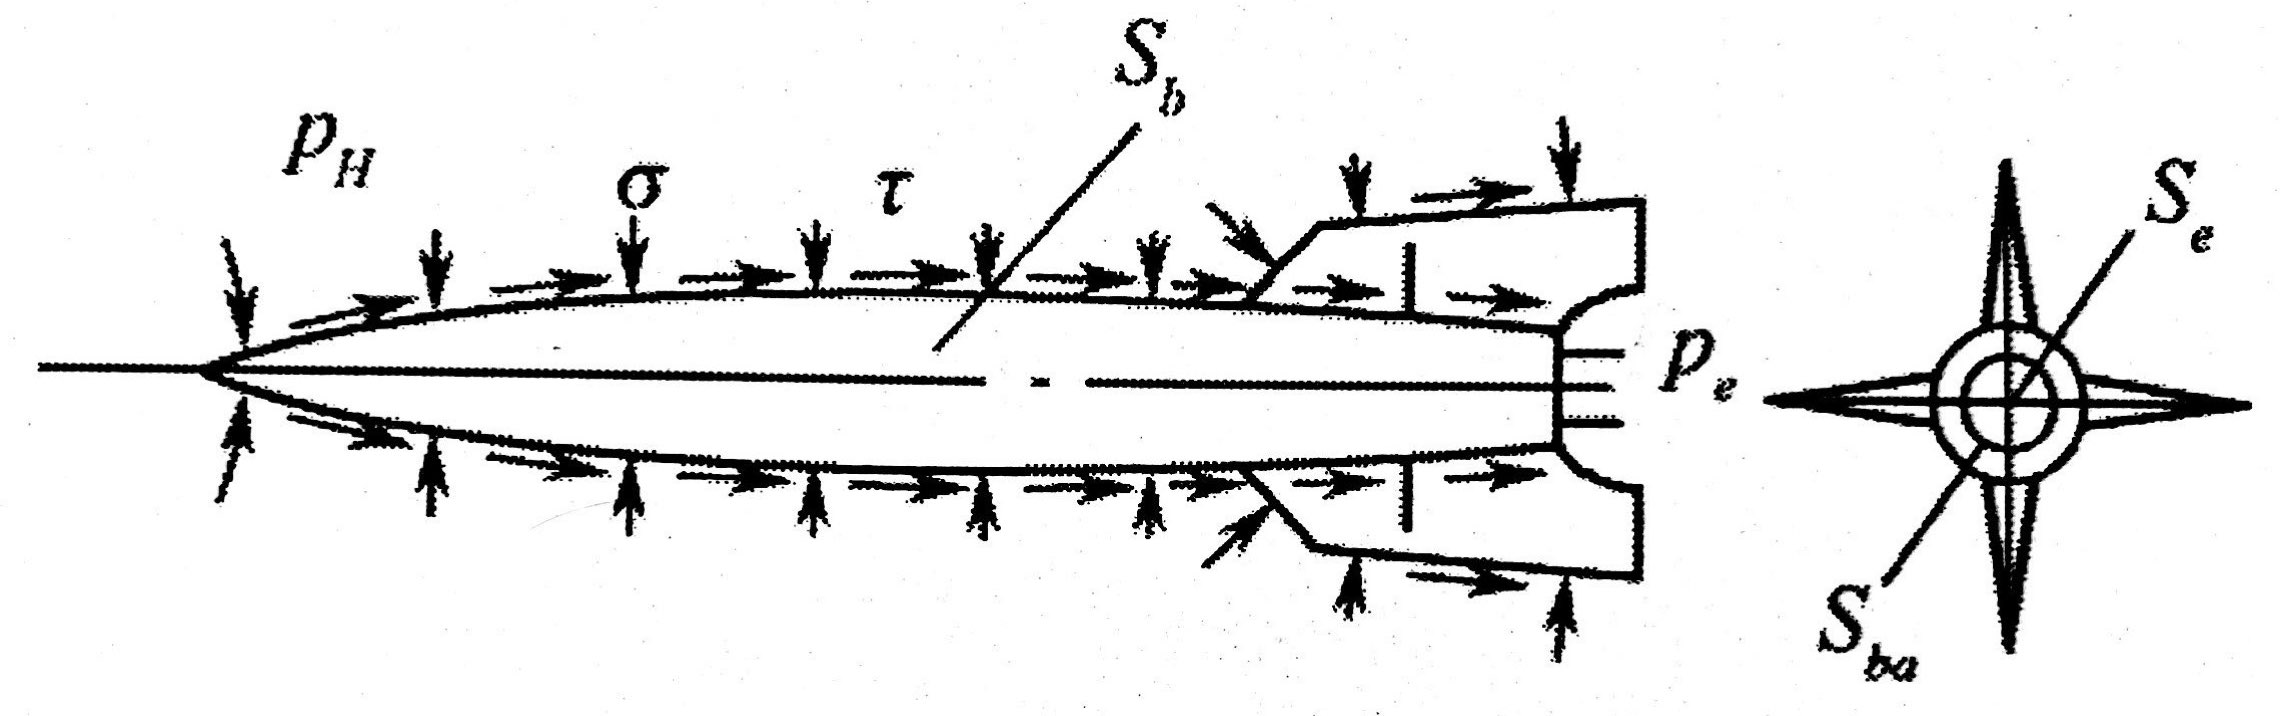
\includegraphics[width=0.6\linewidth]{pic/火箭空气动力.jpg}
	\caption{火箭空气动力}
	\label{火箭空气动力}
\end{figure}

将火箭表面分成喷口截面积$S_e$及除$S_e$以外的弹体表面$S_b$两部分。记空气作用在火箭体表面上单位面积法向力和切向力$\bm{\sigma},\bm{\tau}$,则在$S_b$的每一个微小面积$\d S$上作用有法向力$\bm{\sigma} \d S$记切向力$\bm{\tau} \d S$,因而空气作用在$S_b$上合力为
\begin{equation}
	\bm{R}_b = \int_{S_b} \bm{\sigma}\, \d S + \int_{S_b} \bm{\tau}\, \d S
\end{equation}
同样,当发动机不工作时,空气作用于喷口截面$S_e$上的合力为
\begin{equation}
	\bm{R}_e = \int_{S_e} \bm{\sigma}\, \d S + \int_{S_e}\bm{\tau}\, \d S
\end{equation}

由于法向力$\bm{\sigma}$可以写成未扰动空气的静压$\bm{p}_{H}$与法向剩余压力$\bm{\sigma}'$之和,即
\begin{equation}
	\bm{\sigma} = \bm{p}_H + \bm{\sigma}'
\end{equation}
故空气作用在火箭上的总的合力可写为
\begin{equation}
	\bm{R} = \int_{S_b}\bm{p}_H \, \d S + \int_{S_e}\bm{p}_H \, \d S + \int_{S_b}\bm{\sigma}'\, \d S + \int_{S_e} \bm{\sigma}' \, \d S + \int_{S_b} \bm{\tau}_b \, \d S + \int_{S_e} \bm{\tau}_e \, \d S
\end{equation}
其中前两项为作用在火箭上的空气静压力,在发动机不工作时为0,最后一项为喷口截面上的切应力,一般可忽略。即简化为
\begin{equation}
	\bm{R} = \int_{S_b}\bm{\sigma}'\, \d S + \int_{S_e} \bm{\sigma}' \, \d S + \int_{S_b} \bm{\tau}_b \, \d S 
\end{equation}

即火箭底部面积$S_{ba}$与截面积之差为$S_r$,则
\begin{equation}
	S_e = S_{ba} - S_r
\end{equation}
则可以得到

\theorem[火箭空气动力]
{
	\quad \vspace*{-1em}
	\begin{equation}
		\bm{R} = \int_{S_b - S_r} \bm{\sigma}' \, \d S + \int_{S_b} \bm{\tau}\, \d S + \int_{S_{ba}} \bm{\sigma}'\, \d S
	\end{equation}
	\noindent 其中,
	\begin{enumerate}[\hspace*{1.5em}]
		\item $\displaystyle \int_{S_{ba}} \bm{\sigma}' \, \d S$ \quad \dy[火箭底阻]{HJD},其合力作用线与火箭纵轴$x_1$重合,记为$\bm{X}_{1ba}$\vspace*{-0.5em}
		\item $\displaystyle \int_{S_{b}} \bm{\tau} \, \d S$ \quad 摩擦阻力,其合力作用线与$x_1$重合,记为$\bm{X}_{1f}$
		\item 将$\displaystyle \int_{S_b - S_r} \bm{\sigma}'\, \d S$分解为火箭箭体坐标轴的三个方向,分别为压差阻力$\bm{X}_{1b}$、法向力$\bm{Y}_1$及横向力$\bm{Z}_1$
	\end{enumerate}
	则火箭空气动力方程进一步可以写为
	\begin{equation}
		\bm{R} = \bm{X}_{1ba}+\bm{X}_{1f} + \bm{X}_{1b} + \bm{Y}_1 + \bm{Z}_1
	\end{equation}
	记总的轴向力
	\begin{equation}
		\bm{X}_1 = \bm{X}_{1ba}+\bm{X}_{1f} + \bm{X}_{1b} 
	\end{equation}
	则
	\begin{equation}
		\bm{R} = \bm{X}_1 + \bm{Y}_1 + \bm{Z}_1
	\end{equation}
}

当发动机工作时,在计算发动机推力中,已经将大气静压力$\displaystyle \int_{S_b}\bm{p}_H \, \d S$与发动机喷口截面上的燃气压力

\noindent $\displaystyle \int_{S_e} \bm{p}\, \d S$合成为推力静分量(见\peref[静推力]),计入发动机推力之中。而此时火箭的底阻仅为底部圆环部\\[0.5em]
分的面积$S_r$的法向剩余压力造成。所以,发动机工作与否,总气动力表达式相同。

\clearpage

\noindent \textbf{2. 气动力的工程计算方法}

火箭相对大气运动时,确定气动力是非常复杂的,很难直接通过理论准确确定,目前主要是用\textbf{空气动力学理论进行计算结合空气动力实验校正的方法}。

实际研制过程中,利用上面的方法,通常给出火箭空气动力计算所需的图表与曲线,利用这些曲线即可确定气动力与气动力矩。
\vspace*{0.8em}

\noindent \textbf{3. 气动力在体系内的分解}

实际应用中,气动力的计算采用如下公式:
\begin{equation}
	\begin{cases}
		\, X_1 = C_{x1}\dfrac{1}{2}\rho v^2 S_M = C_{x1}qS_M\\[1em]
		\, Y_1 = C_{y1}\dfrac{1}{2}\rho v^2 S_M = C_{y1}qS_M\\[1em]
		\, Z_1 = C_{z1}\dfrac{1}{2}\rho v^2 S_M = C_{z1}qS_M
	\end{cases}
	\label{气动力1}
\end{equation}
\noindent 其中,
\vspace*{0.5em}

\begin{minipage}{0.5\linewidth}
	\begin{enumerate}[]
		\item $v$ \quad 火箭相对于大气的速度\vspace*{-0.5em}
		\item $\rho$ \quad 大气密度\vspace*{-0.5em}
		\item $S_M$ \quad 火箭最大横截面积,也称为\dy[特征面积]{TZMJ}\vspace*{-0.5em}
		\item $q$ \quad 速度头(\dy[动压头]{DYT}) $q = \dfrac{1}{2} \rho v^2$ \vspace*{-0.5em}
	\end{enumerate}
\end{minipage}
\begin{minipage}{0.5\linewidth}
	\begin{enumerate}[]
		\item $C_{x1}$ \quad \dy[轴向力系数]{ZXLXS}\vspace*{-0.5em}
		\item $C_{y1}$ \quad \dy[法向力系数]{FXLXS}\vspace*{-0.5em}
		\item $C_{z1}$ \quad \dy[横向力系数]{HXLXS}
		\item
	\end{enumerate}
\end{minipage}
\vspace*{1em}

在研究火箭运动规律时,也常常在速度坐标系中讨论,所以空气动力也可以分解为
\begin{equation}
	\bm{R} = \bm{X} + \bm{Y} + \bm{Z}
\end{equation}
各个分量为
\begin{equation}
	\begin{cases}
		\, X = C_{x}\dfrac{1}{2}\rho v^2 S_M = C_{x}qS_M\\[1em]
		\, Y = C_{y}\dfrac{1}{2}\rho v^2 S_M = C_{y}qS_M\\[1em]
		\, Z = C_{z}\dfrac{1}{2}\rho v^2 S_M = C_{z}qS_M
	\end{cases}
	\label{气动力2}
\end{equation}
\noindent 其中,
\vspace*{0.5em}

\begin{minipage}{0.5\linewidth}
	\begin{enumerate}[]
		\item $\bm{X}$ \quad \dy[阻力]{ZL}\vspace*{-0.5em}
		\item $\bm{Y}$ \quad \dy[升力]{SL}\vspace*{-0.5em}
		\item $\bm{Z}$ \quad \dy[侧力]{CL}\vspace*{-0.5em}
	\end{enumerate}
\end{minipage}
\begin{minipage}{0.5\linewidth}
	\begin{enumerate}[]
		\item $C_{x}$ \quad \dy[阻力系数]{ZXLXS}\vspace*{-0.5em}
		\item $C_{y}$ \quad \dy[升力系数]{FXLXS}\vspace*{-0.5em}
		\item $C_{z}$ \quad \dy[侧力系数]{HXLXS}
	\end{enumerate}
\end{minipage}
\vspace*{1em}

利用公式\eqref{气动力1},\eqref{气动力2}求得的$X,X_1$均为正值,而实际合力投影到相应坐标轴是负值,所以需要加上负号,根据速度坐标系与箭体坐标系之间的转换关系,可以得到
\begin{equation}
	\begin{bmatrix}
		-X \\
		Y \\
		Z
	\end{bmatrix}
	=
	\bm{V}_B
	\begin{bmatrix}
		-X_1 \\
		Y_1 \\
		Z_1
	\end{bmatrix}
	\label{气动转换}
\end{equation}
其中,
\begin{equation}
	\bm{V}_B = 
	\begin{bmatrix}
		\cos \beta \cos \alpha & - \cos \beta \sin \alpha & \sin \beta \\
		\sin \alpha & \cos \alpha & 0 \\
		- \sin \beta \cos \alpha & \sin \beta \sin \alpha & \cos \beta
	\end{bmatrix}
\end{equation}

\noindent \textbf{【  阻力和阻力系数  】}

由公式\eqref{气动转换},可以得到
\begin{equation}
	X = X_1 \cos \beta \cos \alpha + Y_1 \cos \beta \sin \alpha - Z_1 \sin \alpha
\end{equation}








